%\documentclass[english]{beamer}
\documentclass[english,hangout]{beamer}
%\documentclass[aspectratio=169]{beamer}
%\usepackage{amsmath}
%\usepackage{amssymb}
\usepackage{rotating}
\usepackage{verbatim}
\usepackage{latexsym}
\usepackage{graphicx}
\usepackage{tabularx}
\usepackage{ragged2e}
\usepackage{eurosym}   % Euro symbol: \euro
\usepackage{listings}
\usepackage{multirow}
\usepackage{colortbl}
\usepackage{textcomp}  % many special symbols
\usepackage{lmodern}
\usepackage{times}
\usepackage[T1]{fontenc}
\usepackage[utf8]{inputenc}
\usepackage[english]{babel}
\usepackage{booktabs}

\colorlet{punct}{red!60!black}
\definecolor{background}{HTML}{EEEEEE}
\definecolor{delim}{RGB}{20,105,176}
\colorlet{numb}{magenta!60!black}

\lstdefinelanguage{json}{
    basicstyle=\normalfont\ttfamily,
    numbers=left,
    numberstyle=\scriptsize,
    stepnumber=1,
    numbersep=8pt,
    showstringspaces=false,
    breaklines=true,
    frame=lines,
    backgroundcolor=\color{background},
    literate=
     *{0}{{{\color{numb}0}}}{1}
      {1}{{{\color{numb}1}}}{1}
      {2}{{{\color{numb}2}}}{1}
      {3}{{{\color{numb}3}}}{1}
      {4}{{{\color{numb}4}}}{1}
      {5}{{{\color{numb}5}}}{1}
      {6}{{{\color{numb}6}}}{1}
      {7}{{{\color{numb}7}}}{1}
      {8}{{{\color{numb}8}}}{1}
      {9}{{{\color{numb}9}}}{1}
      {:}{{{\color{punct}{:}}}}{1}
      {,}{{{\color{punct}{,}}}}{1}
      {\{}{{{\color{delim}{\{}}}}{1}
      {\}}{{{\color{delim}{\}}}}}{1}
      {[}{{{\color{delim}{[}}}}{1}
      {]}{{{\color{delim}{]}}}}{1},
}

%\usetheme[fb2]{FrankfurtUniversity}
\usetheme[fb2,noslogan]{FrankfurtUniversity}
%\slogan{\large\color{red}UNAUTHORIZED}


\title{Blockchain Solution to\\Healthcare Record System using\\Hyperledger Fabric}
\subtitle{Sprint 2 review}
\author{Team Lithium}
%\institute{Frankfurt University of Applied Sciences\\}
\date{\today}%{November 24, 2020}


\begin{document}


\begin{frame}
\titlepage
\end{frame}
%\addtocounter{framenumber}{-1}



\begin{frame}
   \frametitle{Agenda}
   \tableofcontents%[hideallsubsections]
\end{frame}




\section{Sprint 2}

\subsection{Results}

\begin{frame}[fragile]
 \frametitle{Sprint 2}
 \framesubtitle{Results - Overview}
  \begin{itemize}
    \item Development of REST APIs to interact with smart contracts using Fabric SDK.
    \item Finalised patient' data to be used as personal and medical details.
    \item Smart contracts updated with functions like, search based on first and last name, and to get patients' medical history.
    \item Addition of additional peers to the organisation.
    \item UI templates design.
    \item Detailed security analysis of assets.
  \end{itemize}
\end{frame}

\begin{frame}[fragile]
 \frametitle{Sprint 2}
 \framesubtitle{Pending Tasks}
\begin{center}
        \vspace{-1.2em}
            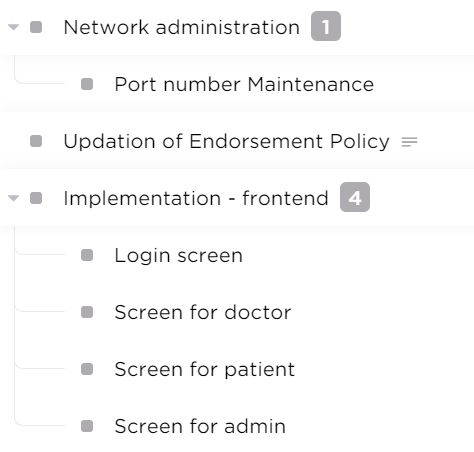
\includegraphics[height=6cm]{pending.JPG}
        \end{center}
\end{frame}

\begin{frame}[fragile]
 \frametitle{Sprint 2}
    \begin{center}
        \vspace{-1.2em}
            Demo
        \end{center}
\end{frame}

% START: JATHIN

\subsection{Secured asset transfer in Fabric}

\begin{frame}[fragile]
    \frametitle{Secured asset transfer in Fabric}
    \framesubtitle{Granting Permission to Doctors}
    \begin{lstlisting}[language=json,firstnumber=1]
{
    'firstName': 'Johannes',
    'lastName': 'Schmidt',
    'age': '23',
    ....
    'bloodGroup': 'B+',
    'allergies': 'No',
    'symptoms': 'Dizziness, Nausea, diastolic',
    ....
    'permissionGranted': 
        ['HOSP001-DOC001', 'HOSP002-DOC002']
}    
    \end{lstlisting}
\end{frame}

\begin{frame}[fragile]
    \frametitle{Secured asset transfer in Fabric}
    \framesubtitle{Two Chaincodes - Doctor Chaincode, Patient Chaincode}
    \begin{center}
        \vspace{-1.2em}
            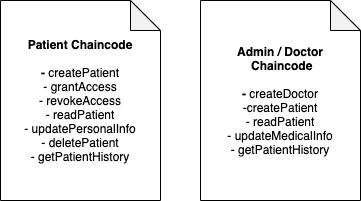
\includegraphics[height=4cm]{Smart-Contracts (1).png}
        \end{center}
        \vspace{-3mm}
\end{frame}


\begin{frame}[fragile]
    \frametitle{Secured asset transfer in Fabric}
    \framesubtitle{Private Channel}
    \begin{center}
        \vspace{-1.2em}
            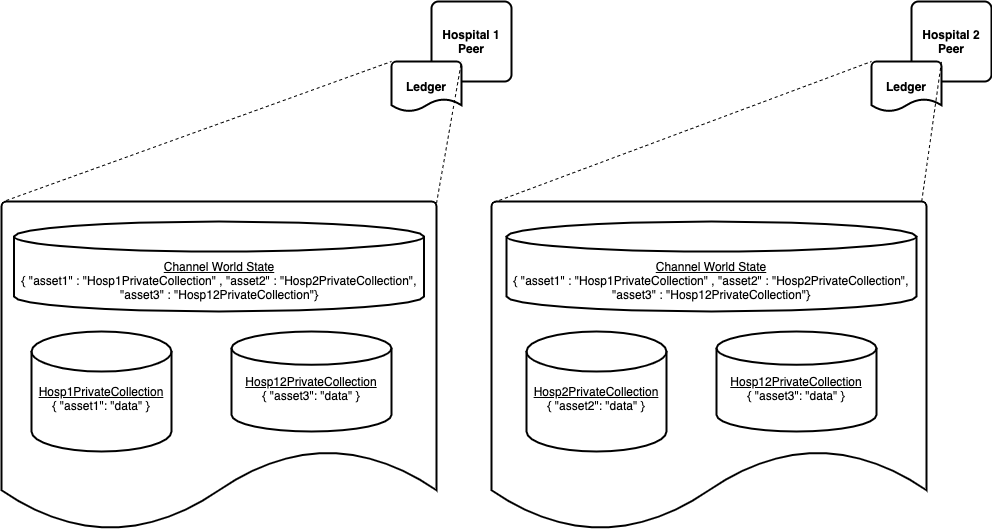
\includegraphics[height=5cm]{PrivateChannel.png}
        \end{center}
        \vspace{-3mm}
\end{frame}

% END: JATHIN

\subsection{Encryption mechanism for the security of assets}
\begin{frame}[fragile]
 \frametitle{Encryption approach}
  \begin{itemize}
  \item As blockchain assets are patients, patient information should have the following details. 
    \begin{lstlisting}[language=json,firstnumber=1]
    {
    "patientId": "p1",
    "password": hash(pwd),
    "firstName": "######",
    "lastName" "######",
    "data": encrypted patient data,
    "requestedAccess": [doctorId1: doctor1's public key, doctorId2: doctor2's public key, ...],
    "permissionGranted": [doctorId1: re-encrypted key for doctor 1, doctorId1: re-encrypted key for doctor 1, ...],
    "encryptedSymmetricKey" : "######"
    }    
    \end{lstlisting}
    \end{itemize}
\end{frame}

\begin{frame}[fragile]
 \frametitle{Encryption approach}
  \begin{itemize}
    \item Patient data will somewhat look like this
    \begin{lstlisting}[language=json,firstnumber=1]
    {
    "address": "",
    "blood group": "",
    "dob": "",
    .
    .
    .
    }
    \end{lstlisting}
  \end{itemize}
\end{frame}

\begin{frame}[fragile]
\frametitle{Encryption approach}
\begin{itemize}
    \item When a patient gets created, the patient's keys(public and private) get stored in the wallet. Patient data will be encrypted by the symmetric key (randomly generated or not yet decided how) and the symmetric key will be encrypted by the patient's public key.
    \item Patient login portal: 
    First-time login = Patient enter patientId -> get ask to create password -> hash value will be generated and stored in ledger -> patient's data will be retrieved and decrypted by patient's private key and then data will be decrypted by a symmetric key
    Further logins = Patient enter patientId -> get ask to enter password -> hash of entered password will be compared with stored one -> patient's data will be retrieved and decrypted by patient's private key and then data will be decrypted by a symmetric key
    
\end{itemize}
\end{frame}

\begin{frame}[fragile]
\frametitle{Encryption approach}
\begin{itemize}
    \item Doctors will be treated as users as well and info will be stored in the wallet. For the successful login of doctors, credentials will be stored on a local database.
    \item Doctors login portal: Doctor need to select the hospital he/she belong -> Doctor will enter username and pwd -> once authenticated, can view all patients in the network (can see only id, firstName and lastName) as a list which will have 'request access' button on every entry at last.
    \item Patient can see the list of doctors who requested for the access on the portal. If the patient grants the permission to a doctor then re-encryption key will be generated (this is a combination of the patient's private key and doctor's public key who requested access).
\end{itemize}
\end{frame}

\begin{frame}[fragile]
\frametitle{Encryption approach}
\begin{itemize}
    \item Doctor can view a patient's data now by following steps:-
    a) Encrypt the encryptedSymmetricKey by re-encryption key - encrypted the cipher,
    b) Decrypt the encrypted cipher by own private key - symmetric key, and 
    c) Decrypt patient data by a symmetric key
    \item Admin: Create a patient as a user, generate patient data and doctor as a user.
    \item Advantages:
    a) Peers can't read the patient's data as it is encrypted. 
    b) Modifications are only possible by smart contracts.
\end{itemize}
\end{frame}


\section{Sprint 3}

\begin{frame}[fragile]
 \frametitle{Sprint 3}
 \framesubtitle{Tasks}
    \begin{center}
        \vspace{-1.2em}
            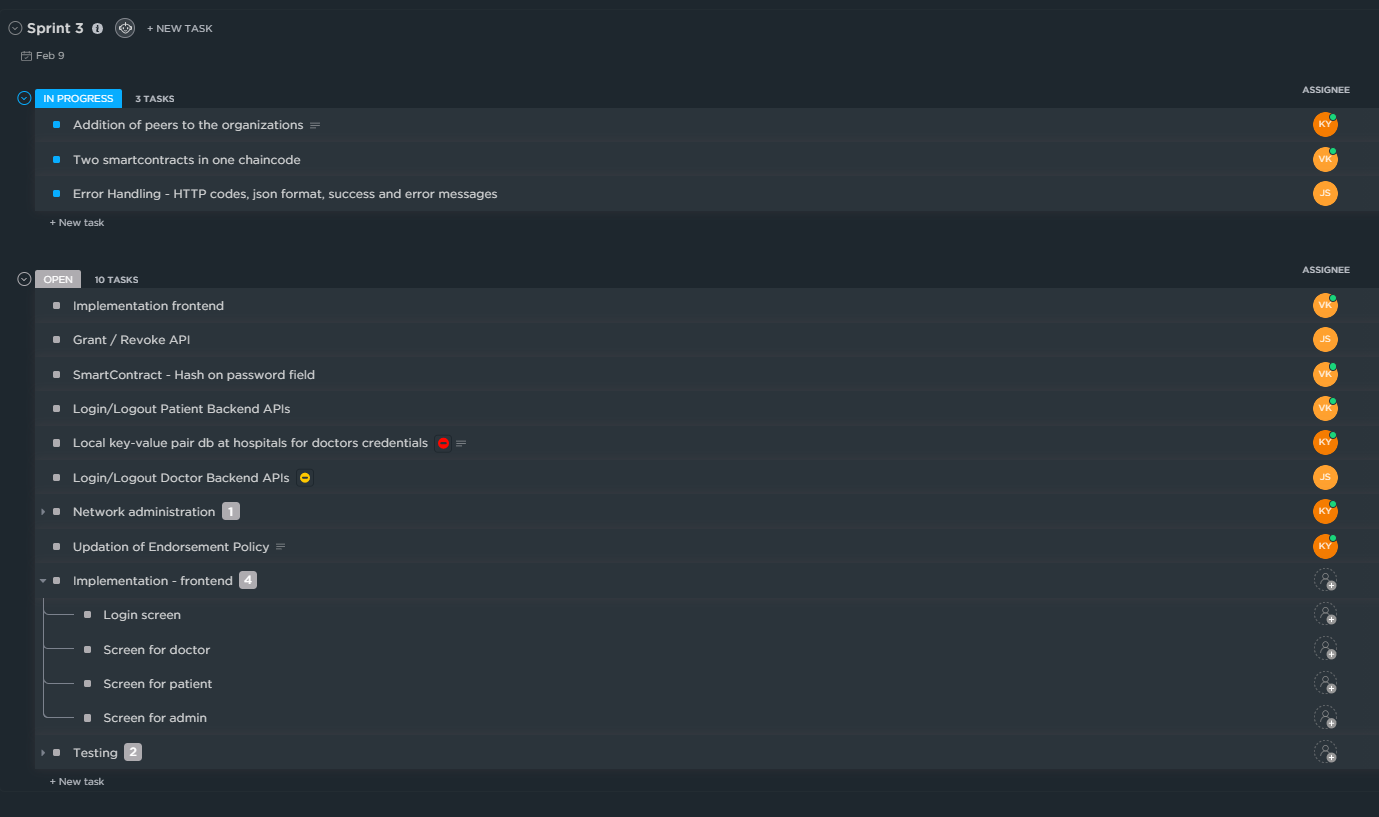
\includegraphics[height=7cm]{sprint 3_tickets.PNG}
        \end{center}
%\tiny Source: \texttt{https://hyperledger-fabric.readthedocs.io/en/latest/txflow.html}
\end{frame}



\section{References}

\begin{frame}
\frametitle{References}
\begin{thebibliography}{00}
\bibitem{b1} https://www.ncbi.nlm.nih.gov/pmc/articles/PMC7010942/
\bibitem{b2} https://www.ncbi.nlm.nih.gov/pmc/articles/PMC7474412/
\bibitem{b3} https://www.sciencedirect.com/science/article/pii/S2214212-619306155
\bibitem{b4} https://hyperledger-fabric.readthedocs.io/ Accessed-On:12/01/2021
\bibitem{b5} https://medium.com/@lichunshen84/build-a-blockchain-poc-application-using-hyperledger-fabric-5a32687072b7, Accessed-On:01/12/2020
\end{thebibliography}

\end{frame}


\end{document}